% ==========================================================================
\section{Language F: Euler/Venn diagrams and bag-and-arrow pictures}
\label{sec:euler}

\paragraph{Marks.} Closed blobs (sets), dots (elements), arrows between dots (values of a
function).
\paragraph{Legal moves.} Containment and overlap of blobs; chaining of arrows.
\paragraph{Soundness.} For \emph{finitely many} blobs, an Euler diagram is a faithful
picture of the Boolean algebra they generate, and validity of a syllogism can be decided
by drawing (this is a theorem about Venn diagrams). Bag-and-arrow pictures are exact for
statements about injectivity and surjectivity, because those notions are literally about
arrow patterns.

\begin{figure}[H]
\centering
\begin{tikzpicture}[x=1cm,y=1cm]
 \foreach \k/\lab/\ttl in {0/{a}/{injective, not surjective},
                           4.6/{b}/{surjective, not injective},
                           9.2/{c}/{bijective}}{
  \begin{scope}[xshift=\k cm]
    \draw[thick] (0,0) ellipse (0.6 and 1.25);
    \draw[thick] (2.4,0) ellipse (0.6 and 1.25);
    \node[font=\scriptsize] at (1.2,-1.75) {\ttl};
  \end{scope}}
 % injective not surjective
 \foreach \y in {0.7,0,-0.7} {\fill (0,\y) circle (1.5pt);}
 \foreach \y in {0.9,0.3,-0.3,-0.9} {\fill (2.4,\y) circle (1.5pt);}
 \draw[-{Stealth[length=1.6mm]}] (0.1,0.7) -- (2.3,0.9);
 \draw[-{Stealth[length=1.6mm]}] (0.1,0) -- (2.3,0.3);
 \draw[-{Stealth[length=1.6mm]}] (0.1,-0.7) -- (2.3,-0.3);
 % surjective not injective
 \begin{scope}[xshift=4.6cm]
 \foreach \y in {0.9,0.3,-0.3,-0.9} {\fill (0,\y) circle (1.5pt);}
 \foreach \y in {0.7,0,-0.7} {\fill (2.4,\y) circle (1.5pt);}
 \draw[-{Stealth[length=1.6mm]}] (0.1,0.9) -- (2.3,0.7);
 \draw[-{Stealth[length=1.6mm]}] (0.1,0.3) -- (2.3,0.7);
 \draw[-{Stealth[length=1.6mm]}] (0.1,-0.3) -- (2.3,0);
 \draw[-{Stealth[length=1.6mm]}] (0.1,-0.9) -- (2.3,-0.7);
 \end{scope}
 % bijective
 \begin{scope}[xshift=9.2cm]
 \foreach \y in {0.7,0,-0.7} {\fill (0,\y) circle (1.5pt);}
 \foreach \y in {0.7,0,-0.7} {\fill (2.4,\y) circle (1.5pt);}
 \draw[-{Stealth[length=1.6mm]}] (0.1,0.7) -- (2.3,0.7);
 \draw[-{Stealth[length=1.6mm]}] (0.1,0) -- (2.3,0);
 \draw[-{Stealth[length=1.6mm]}] (0.1,-0.7) -- (2.3,-0.7);
 \end{scope}
\end{tikzpicture}
\caption{Exercise 2.2 in pictures. \emph{Injective} = no two arrows land on the same dot;
\emph{surjective} = no dot on the right is missed; \emph{bijective} = a perfect matching,
which is exactly the situation in which the arrows may be reversed. Reversing the arrows
of the third picture \emph{is} the inverse function -- the same content as
Figure~\ref{fig:invunique}, in a picture a first-year student can draw in three seconds.}
\label{fig:bags}
\end{figure}

\begin{figure}[H]
\centering
\begin{tikzpicture}[x=1cm,y=1cm]
  \foreach \k in {0,2.6,5.2}{\draw[thick] (\k,0) ellipse (0.55 and 1.15);}
  \foreach \y in {0.6,0,-0.6} {\fill (0,\y) circle (1.5pt);}
  \foreach \y in {0.85,0.28,-0.28,-0.85} {\fill (2.6,\y) circle (1.5pt);}
  \foreach \y in {0.9,0.3,-0.3,-0.9} {\fill (5.2,\y) circle (1.5pt);}
  \draw[-{Stealth[length=1.6mm]},blue!60!black] (0.1,0.6) -- (2.5,0.85);
  \draw[-{Stealth[length=1.6mm]},blue!60!black] (0.1,0) -- (2.5,0.28);
  \draw[-{Stealth[length=1.6mm]},blue!60!black] (0.1,-0.6) -- (2.5,-0.85);
  \draw[-{Stealth[length=1.6mm]},red!60!black] (2.7,0.85) -- (5.1,0.9);
  \draw[-{Stealth[length=1.6mm]},red!60!black] (2.7,0.28) -- (5.1,-0.3);
  \draw[-{Stealth[length=1.6mm]},red!60!black] (2.7,-0.28) -- (5.1,0.3);
  \draw[-{Stealth[length=1.6mm]},red!60!black] (2.7,-0.85) -- (5.1,-0.9);
  \node[font=\scriptsize,blue!60!black] at (1.3,1.45) {$g$};
  \node[font=\scriptsize,red!60!black] at (3.9,1.45) {$f$};
  \draw[-{Stealth[length=1.8mm]},thick,dashed] (0.15,-1.45) .. controls (2.6,-2.1) ..
      (5.05,-1.45);
  \node[font=\scriptsize] at (2.6,-2.25) {$f\circ g$};
\end{tikzpicture}
\caption{Exercise 2.18: if no two blue arrows collide and no two red arrows collide, then
no two dashed composites collide. The picture \emph{is} the proof, and it is faithful --
this is one of the cases where the bag-and-arrow language is certified. Certified in
\lean{DiagramProofs.injective\_comp}.}
\label{fig:injcomp}
\end{figure}

\begin{figure}[H]
\centering
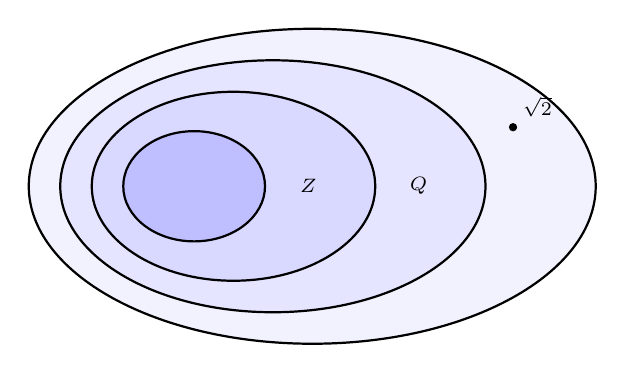
\begin{tikzpicture}[x=1cm,y=1cm]
  \draw[thick,fill=blue!5]  (0,0) ellipse (3.6 and 2.0);
  \draw[thick,fill=blue!10] (-0.5,0) ellipse (2.7 and 1.6);
  \draw[thick,fill=blue!15] (-1.0,0) ellipse (1.8 and 1.2);
  \draw[thick,fill=blue!25] (-1.5,0) ellipse (0.9 and 0.7);
  \node[font=\scriptsize] at (-1.5,0) {$\N$};
  \node[font=\scriptsize] at (-0.05,0) {$\mathbb{Z}$};
  \node[font=\scriptsize] at (1.35,0) {$\mathbb{Q}$};
  \node[font=\scriptsize] at (2.9,0) {$\R$};
  \fill (2.55,0.75) circle (1.5pt) node[font=\scriptsize,above right]{$\sqrt2$};
\end{tikzpicture}
\caption{Exercise 1.3: the number systems as an Euler diagram. The single dot placed in
the outermost ring is exercise 1.9, ``$\sqrt2$ is irrational'' -- and it is the one thing
the picture cannot prove. A diagram can \emph{record} a classification; only an argument
can \emph{establish} membership.}
\label{fig:venn}
\end{figure}

\begin{trap}[Blobs presuppose sets]
Exercise 1.2 (the shepherd who tends exactly the sheep of those who do not tend their
own -- Russell's paradox) is unanswerable, and no Euler diagram can show this: drawing a
blob already assumes the collection is a set. Likewise 1.1 a), b) (``clever people'',
``beautiful paintings''): the failure is at the level of \emph{whether the blob may be
drawn at all}. Diagrams are silent about their own presuppositions.
\end{trap}

\subsection*{An aside: Peirce's existential graphs}

For pure logic there \emph{is} a complete diagrammatic system: C.\ S.\ Peirce's
existential graphs, with three reversible rules (double cut, insertion/erasure in odd/even
depth, iteration). Statements are written as nested ovals -- an oval is negation, and
juxtaposition is conjunction -- so implication is a double oval.

\begin{figure}[H]
\centering
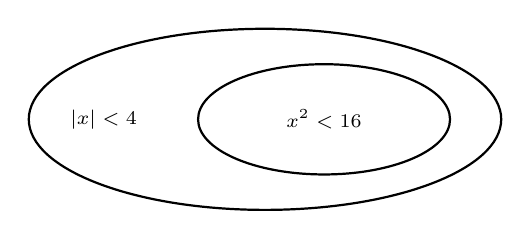
\begin{tikzpicture}[x=1cm,y=1cm]
  \draw[thick] (0,0) ellipse (3.0 and 1.15);
  \draw[thick] (0.75,0) ellipse (1.6 and 0.7);
  \node[font=\scriptsize] at (-2.05,0) {$|x|<4$};
  \node[font=\scriptsize] at (0.75,0) {$x^{2}<16$};
\end{tikzpicture}
\caption{Exercise 1.7 c), ``if $|x|<4$ then $x^{2}<16$'', as an existential graph: the
outer oval negates ``$|x|<4$ and not $x^{2}<16$''. Peirce's rules let one \emph{derive}
consequences by adding and erasing ovals, so this is a genuine, complete, diagram-only
proof system for first-order logic -- historically the first one.}
\label{fig:peirce}
\end{figure}

% ==========================================================================
\section{Language G: order diagrams, and inequalities as paths}
\label{sec:hasse}

\paragraph{Marks.} Nodes, edges drawn upwards (``$\le$'').
\paragraph{Legal moves.} Follow a path upwards: composition of $\le$'s is transitivity.
\paragraph{Soundness.} Total, because a preordered set \emph{is} a category with at most
one arrow between any two objects. Drawing a chain of estimates and reading off the
endpoints is exactly composing morphisms.

\begin{figure}[H]
\centering
\begin{tikzcd}[row sep=small, column sep=tiny]
 & & \sum_{i<n}|a_i| \\
 & \Bigl|\sum_{i<n-1}a_i\Bigr|+|a_{n-1}| \arrow[ur,dash] & \\
\Bigl|\sum_{i<n}a_i\Bigr| \arrow[ur,dash] & &
\end{tikzcd}
\qquad
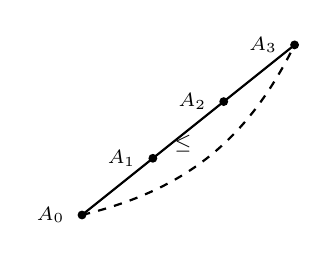
\begin{tikzpicture}[x=1cm,y=0.9cm,baseline=(current bounding box.center)]
  \foreach \i/\lab in {0/{A_0},1/{A_1},2/{A_2},3/{A_3}}{
    \fill (0.9*\i,0.8*\i) circle (1.6pt);
    \node[font=\scriptsize,anchor=east] at (0.9*\i-0.1,0.8*\i) {$\lab$};}
  \foreach \i in {0,1,2}{
    \draw[thick] (0.9*\i,0.8*\i) -- (0.9*\i+0.9,0.8*\i+0.8);}
  \draw[thick,dashed,bend right=25] (0,0) to (2.7,2.4);
  \node[font=\scriptsize,anchor=west] at (1.05,1.0) {$\le$};
\end{tikzpicture}
\caption{A chain of estimates is a path in a Hasse diagram: each edge is one inequality,
the path is their composite. In this language the ``generalised triangle inequality''
(exercise 1.13) is a walk of length $n$, and the induction that proves it is the
observation that a walk is built one edge at a time -- exactly
\lean{TriangleOverlap.dist\_chain}. Exercise 1.15 c) (the sandwich
$2\sqrt{n+1}-2<\sum 1/\sqrt i<2\sqrt n-1$) is the same picture with two paths, one on
each side.}
\label{fig:hasse}
\end{figure}

The order-theoretic reading is also what makes the metric/enrichment story of
Section~\ref{sec:catdiag} precise: the poset $([0,\infty),\ge)$ with $+$ is the place
where the hom-objects live, so an inequality between distances is an arrow of that poset,
and the triangle inequality is the composition law.

% ==========================================================================
\section{Language H: optimisation by superposition}
\label{sec:optim}

\paragraph{Marks.} Two figures of the same kind, drawn on top of each other.
\paragraph{Legal moves.} Compare areas or lengths after superposition; complete a square.
\paragraph{Soundness.} None; the residue is that the comparison holds for \emph{every}
member of the family, not just the drawn one. Usually the residue is a completed square.

\begin{figure}[H]
\centering
\begin{tikzpicture}[x=0.34cm,y=0.34cm]
  \fill[blue!12] (0,0) rectangle (14,6);
  \draw[thick] (0,0) rectangle (14,6);
  \draw[thick,red!70!black] (0,0) rectangle (10,10);
  \draw[pattern=north east lines,pattern color=red!40] (10,0) rectangle (14,6);
  \node[font=\scriptsize] at (7,3.0) {$x(20-x)$};
  \node[font=\scriptsize,red!70!black,anchor=south] at (5,10.3) {$10\times10$};
  \draw[decorate,decoration={brace,amplitude=4pt,mirror}] (0,-0.5) -- (14,-0.5)
     node[midway,below,font=\scriptsize]{$x$};
  \draw[decorate,decoration={brace,amplitude=4pt}] (-0.5,0) -- (-0.5,6)
     node[midway,left,font=\scriptsize]{$20-x$};
\end{tikzpicture}
\caption{Exercise 4.11 a): split $20$ into two summands of largest product. Superimpose
the rectangle $x\times(20-x)$ on the square $10\times10$: the part of the rectangle
sticking out is congruent to a strip missing from the square, and the square keeps one
extra corner square of side $|x-10|$. Hence $x(20-x)=100-(x-10)^{2}\le100$, with equality
only for $x=10$: no derivative is needed. Certified in
\lean{DiagramProofs.split\_twenty\_max\_product}. Exercises 4.12, 4.14 and 4.15 are the
same move with a sector, a circumscribed triangle, and a rectangle under a parabola.}
\label{fig:optsq}
\end{figure}
